\newpage
\subsubsection{DJI Air 2s}
\begin{wrapfigure}{r}{0.3\textwidth}
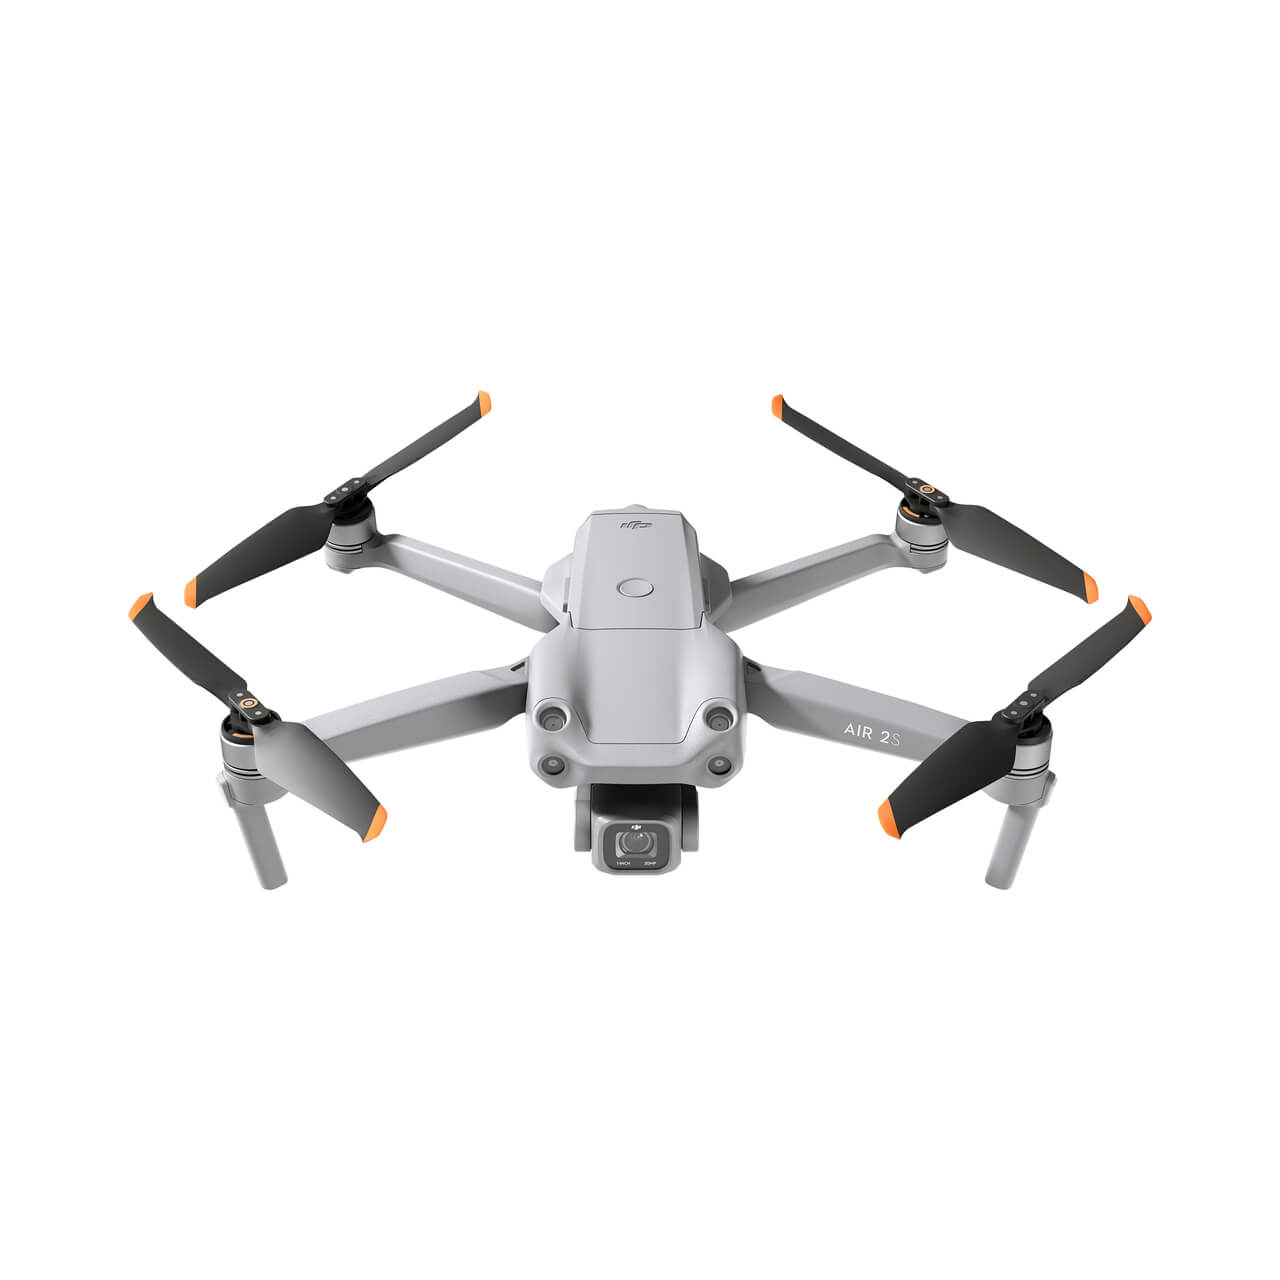
\includegraphics[width=1\linewidth]{uav/models/51_air2s.jpg}
\caption{Air 2S}
\end{wrapfigure}
The Air 2S \cite{phantom4} is DJI's current flagship prosumer drone. While there have been several variants of this popular drone, like the V2.0 Pro, they are identical to our requirements.

\paragraph{Payload capacity}\mbox{Score: 0} \\
While DJI only notes payload capacity on the Matrice 300 Series, the payload capacity of the Phantom 4 is generally considered to be 400 grams. \cite{air2spayloadrelease} This is beneath our minimum requirement of payload capacity.

\paragraph{Mounting clearance}\mbox{Score: 1.0} \\
The Air 2S is a small drone. Due to it's popularity, there does exist  has several third party mounting solutions that one can buy \cite{air2spayloadrelease} or build themselves \cite{thingiverseair}. One could easily use these mounting solutions to mount sensors or water collectors.

\paragraph{Navigation/Routing}\mbox{Score: 1.5} \\
One can plan routes for the Air 2S using the latest DJI Fly app \cite{djifly} available on iOS and Android. There is also the excellent DroneExpert search and rescue flight app available on iOS which is designed to pre-program an ideal flight route. \cite{desar}

\paragraph{Flight time}\mbox{Score: 1.5} \\
The flight time of the Air 2S is 30 minutes, well passing the minimum required flight time.

\paragraph{Range}\mbox{Score: 1.5} \\
The maximum radio range is 12.0km, well over the minimum required range. This also includes image transmission.

\paragraph{Waterproof}\mbox{Score: 1.0} \\
The Air 2S is not waterproof by default, but there are wetsuits available which makes the drone dust-tight and immersible up to 1 meter in water, basically creating it IP67 proof. \cite{air2swetsuit}

\paragraph{Landing in water}\mbox{Score: 0.5} \\
While the Air 2S does not have a water landing gear by default, there are commercial kits one can buy to make the drone able to land on water and give it extra mounting clearance. \cite{air2slandinggear} One could also create their own water landing gear. \cite{diylanding} Because the Air 2S is a smaller drone, it might not be suitable for consistently landing in the water however.

\paragraph{Maneuverability}\mbox{Score: 0.8} \\
The Air 2S is a smaller drone and has the caveats of a smaller drone, being more fragile. It does have the specifications available to go fast, going a maximum of 19m/s.

\paragraph{Total score:}\mbox{0} \\
The Air 2S doesn't seem like a drone suitable for our purposes. The small size makes planned common tasks of the drone quite unstable. It also doesn't meet the payload capacity requirements.